\documentclass[aspectratio=169,12pt]{beamer}

% A self-contained technology-conference keynote deck.
% Compile with: latexmk -pdf -interaction=nonstopmode main.tex

\usepackage[T1]{fontenc}
\usepackage[utf8]{inputenc}
\usepackage{lmodern}
\usepackage{microtype}
\usepackage{amsmath}
\usepackage{booktabs}
\usepackage{array}
\usepackage{listings}
\usepackage{tikz}
\usetikzlibrary{arrows.meta,calc,fit,positioning,shapes.geometric}

% -----------------------------------------------------------------------------
% Visual system
% -----------------------------------------------------------------------------
\definecolor{Ink}{HTML}{07111F}
\definecolor{InkSoft}{HTML}{0D1B2D}
\definecolor{Panel}{HTML}{13243A}
\definecolor{Cloud}{HTML}{F6F8FC}
\definecolor{Mist}{HTML}{A9B6C8}
\definecolor{Cyan}{HTML}{39E6D0}
\definecolor{Blue}{HTML}{5F8BFF}
\definecolor{Orange}{HTML}{FFB45B}
\definecolor{Coral}{HTML}{FF6B78}
\definecolor{Green}{HTML}{75E49A}

\usetheme{default}
\usefonttheme{professionalfonts}
\renewcommand{\familydefault}{\sfdefault}
\setbeamertemplate{navigation symbols}{}
\setbeamertemplate{blocks}[default]
\setbeamersize{text margin left=0.74cm,text margin right=0.74cm}

\setbeamercolor{background canvas}{bg=Ink}
\setbeamercolor{normal text}{fg=Cloud,bg=Ink}
\setbeamercolor{frametitle}{fg=Cloud,bg=Ink}
\setbeamercolor{structure}{fg=Cyan}
\setbeamercolor{itemize item}{fg=Cyan}
\setbeamercolor{itemize subitem}{fg=Blue}
\setbeamercolor{code panel}{fg=Cloud,bg=Panel}
\setbeamerfont{frametitle}{size=\fontsize{35}{39}\selectfont,series=\bfseries}

\setbeamertemplate{itemize item}{\raise0.15ex\hbox{\color{Cyan}\scriptsize$\blacktriangleright$}}
\setbeamertemplate{itemize subitem}{\raise0.15ex\hbox{\color{Blue}\tiny$\bullet$}}

\setbeamertemplate{frametitle}{%
  \nointerlineskip
  \begin{beamercolorbox}[wd=\paperwidth,ht=1.26cm,dp=0.34cm,leftskip=0.74cm,rightskip=0.74cm]{frametitle}
    \usebeamerfont{frametitle}\insertframetitle
  \end{beamercolorbox}%
}

\setbeamertemplate{footline}{%
  \leavevmode
  \hbox{%
    \begin{beamercolorbox}[wd=.78\paperwidth,ht=0.38cm,dp=0.13cm,leftskip=0.74cm]{author in head/foot}%
      \color{Mist}\fontsize{8}{9}\selectfont BEYOND THE DEMO \hspace{0.45em}\textcolor{Cyan}{/}\hspace{0.45em} TECHNOLOGY CONFERENCE KEYNOTE
    \end{beamercolorbox}%
    \begin{beamercolorbox}[wd=.22\paperwidth,ht=0.38cm,dp=0.13cm,rightskip=0.74cm plus 1fil]{date in head/foot}%
      \hfill\color{Mist}\fontsize{9}{10}\selectfont\insertframenumber\hspace{0.35em}\textcolor{Cyan}{/}\hspace{0.35em}\inserttotalframenumber
    \end{beamercolorbox}%
  }%
}

\setlength{\leftmargini}{1.05em}
\setlength{\leftmarginii}{0.95em}
\setlength{\parskip}{0.25em}

% -----------------------------------------------------------------------------
% Reusable typography and drawing helpers
% -----------------------------------------------------------------------------
\newcommand{\eyebrow}[1]{{\color{Cyan}\bfseries\fontsize{11}{13}\selectfont\MakeUppercase{#1}}}
\newcommand{\bodytext}[1]{{\color{Cloud}\fontsize{16}{20}\selectfont #1}}
\newcommand{\mutedtext}[1]{{\color{Mist}\fontsize{14}{18}\selectfont #1}}
\newcommand{\smalllabel}[1]{{\color{Mist}\bfseries\fontsize{11}{13}\selectfont\MakeUppercase{#1}}}
\newcommand{\cyantext}[1]{\textcolor{Cyan}{#1}}
\newcommand{\orange}[1]{\textcolor{Orange}{#1}}
\newcommand{\coral}[1]{\textcolor{Coral}{#1}}

\newcommand{\sectionframe}[2]{%
  \begin{frame}[plain,t]
    \begin{tikzpicture}[remember picture,overlay]
      \fill[Ink] (current page.south west) rectangle (current page.north east);
      \fill[Cyan] ([xshift=0.75cm,yshift=-0.78cm]current page.north west)
        rectangle ++(1.2cm,0.08cm);
      \draw[Blue!40,line width=0.7pt]
        ([xshift=-0.8cm,yshift=0.9cm]current page.south east) circle (2.45cm);
      \draw[Cyan!28,line width=0.7pt]
        ([xshift=-0.8cm,yshift=0.9cm]current page.south east) circle (1.75cm);
    \end{tikzpicture}
    \vspace*{1.2cm}
    \eyebrow{#1}\par\vspace{0.4cm}
    {\color{Cloud}\bfseries\fontsize{43}{48}\selectfont #2\par}
  \end{frame}%
}

\tikzset{
  flowarrow/.style={-{Latex[length=2.5mm,width=1.8mm]},line width=1.2pt,draw=Mist!75},
  thinflow/.style={-{Latex[length=2mm,width=1.4mm]},line width=0.8pt,draw=Mist!60},
  nodebase/.style={rounded corners=2mm,minimum height=1.0cm,align=center,inner xsep=5mm,
    draw=Panel!20,fill=Panel,text=Cloud,font=\fontsize{14}{17}\selectfont\bfseries},
  dot/.style={circle,minimum size=4.5mm,inner sep=0pt,draw=none},
}

\lstdefinestyle{keynote}{
  language=Python,
  basicstyle=\ttfamily\fontsize{12}{14}\selectfont\color{Cloud},
  keywordstyle=\bfseries\color{Cyan},
  commentstyle=\itshape\color{Mist},
  stringstyle=\color{Orange},
  showstringspaces=false,
  columns=fullflexible,
  keepspaces=true,
  aboveskip=0pt,
  belowskip=0pt,
}

\hypersetup{
  pdftitle={Beyond the Demo: Engineering AI Systems That Earn Trust},
  pdfsubject={Technology conference keynote},
  pdfkeywords={AI systems, reliability, evaluation, observability, human control}
}

\title{Beyond the Demo}
\subtitle{Engineering AI systems that earn trust}
\author{Technology Conference Keynote}
\date{2026}

\begin{document}

% -----------------------------------------------------------------------------
% 01 — Title
% -----------------------------------------------------------------------------
\begin{frame}[plain,t]
  \begin{tikzpicture}[remember picture,overlay]
    \fill[Ink] (current page.south west) rectangle (current page.north east);
    \fill[Cyan] ([xshift=0.78cm,yshift=-0.70cm]current page.north west)
      rectangle ++(1.25cm,0.09cm);
    \draw[Blue!38,line width=0.8pt]
      ([xshift=-1.0cm,yshift=0.35cm]current page.south east) circle (3.55cm);
    \draw[Cyan!32,line width=0.8pt]
      ([xshift=-1.0cm,yshift=0.35cm]current page.south east) circle (2.65cm);
    \draw[Orange!35,line width=0.8pt]
      ([xshift=-1.0cm,yshift=0.35cm]current page.south east) circle (1.75cm);
    \fill[Cyan] ([xshift=-1.0cm,yshift=0.35cm]current page.south east) circle (0.10cm);
  \end{tikzpicture}
  \vspace*{0.72cm}
  \eyebrow{Technology Conference Keynote}\par
  \vspace{0.48cm}
  {\color{Cloud}\bfseries\fontsize{54}{56}\selectfont Beyond\par}
  {\color{Cloud}\bfseries\fontsize{54}{56}\selectfont the \cyantext{Demo}\par}
  \vspace{0.46cm}
  {\color{Mist}\fontsize{20}{25}\selectfont Engineering AI systems that earn trust\par}
  \vfill
  {\color{Mist}\fontsize{12}{15}\selectfont SYSTEMS TRACK \hspace{0.55em}\textcolor{Cyan}{/}\hspace{0.55em} 2026}\par
  \vspace*{0.34cm}
\end{frame}

% -----------------------------------------------------------------------------
% 02 — Opening tension
% -----------------------------------------------------------------------------
\begin{frame}[plain]
  \begin{tikzpicture}[remember picture,overlay]
    \fill[Ink] (current page.south west) rectangle (current page.north east);
    \fill[Coral] ([xshift=0.78cm,yshift=-0.72cm]current page.north west)
      rectangle ++(1.25cm,0.09cm);
    \node[anchor=north west,text=Cyan,font=\bfseries\fontsize{11}{13}\selectfont]
      at ([xshift=0.78cm,yshift=-0.98cm]current page.north west) {THE INFLECTION POINT};
    \node[anchor=north west,text=Cloud,align=left,font=\bfseries\fontsize{42}{47}\selectfont]
      at ([xshift=0.78cm,yshift=-1.72cm]current page.north west)
      {The demo is no longer\\the hard part.};
    \node[anchor=north west,text=Mist,align=left,font=\fontsize{18}{22}\selectfont]
      at ([xshift=0.78cm,yshift=-5.02cm]current page.north west)
      {The hard part is knowing what the system will do\\after the applause, under real load, for a real person.};
    \draw[Mist!35,line width=0.8pt]
      ([xshift=0.78cm,yshift=0.78cm]current page.south west) --
      ([xshift=-0.78cm,yshift=0.78cm]current page.south east);
    \fill[Coral] ([xshift=0.78cm,yshift=0.78cm]current page.south west) circle (0.10cm);
    \node[anchor=south west,text=Cloud,font=\fontsize{13}{16}\selectfont\bfseries]
      at ([xshift=1.08cm,yshift=0.97cm]current page.south west) {Prototype};
    \node[anchor=south east,text=Cyan,font=\fontsize{13}{16}\selectfont\bfseries]
      at ([xshift=-0.78cm,yshift=0.97cm]current page.south east) {Production behavior};
  \end{tikzpicture}
\end{frame}

% -----------------------------------------------------------------------------
% 03 — Shape of software
% -----------------------------------------------------------------------------
\begin{frame}{AI reshapes software}
  \vspace{0.10cm}
  \begin{columns}[T,onlytextwidth]
    \begin{column}{0.45\textwidth}
      \eyebrow{Conventional software}\par\vspace{0.32cm}
      {\color{Cloud}\bfseries\fontsize{25}{28}\selectfont
        Specification\\becomes behavior\par}
      \vspace{0.16cm}
      \mutedtext{We debug code-to-output paths against an explicit contract.}
      \vspace{0.12cm}
      
\begin{tikzpicture}[node distance=3mm]
        \node[nodebase,minimum width=1.55cm,inner xsep=2mm] (i) {Input};
        \node[nodebase,minimum width=1.55cm,inner xsep=2mm,right=of i] (c) {Code};
        \node[nodebase,minimum width=1.55cm,inner xsep=2mm,right=of c] (o) {Output};
        \draw[flowarrow] (i) -- (c);
        \draw[flowarrow] (c) -- (o);
      \end{tikzpicture}
    \end{column}
    \hfill
    \begin{column}{0.48\textwidth}
      \eyebrow{AI-native software}\par\vspace{0.32cm}
      {\color{Cloud}\bfseries\fontsize{25}{28}\selectfont
        Intent\\constrains behavior\par}
      \vspace{0.16cm}
      \mutedtext{We engineer boundaries around a range of plausible outputs.}
      \vspace{0.12cm}
      
\begin{tikzpicture}[node distance=3mm]
        \node[nodebase,minimum width=1.55cm,inner xsep=2mm] (i) {Intent};
        \node[nodebase,minimum width=1.65cm,inner xsep=2mm,right=of i,fill=Blue!45!Ink] (m) {Model};
        \node[nodebase,minimum width=2.05cm,inner xsep=2mm,right=of m,fill=Cyan!18!Ink] (g) {Guardrails};
        \draw[flowarrow] (i) -- (m);
        \draw[flowarrow] (m) -- (g);
      \end{tikzpicture}
    \end{column}
  \end{columns}
\end{frame}

% -----------------------------------------------------------------------------
% 04 — Two loops
% -----------------------------------------------------------------------------
\begin{frame}{Products run two loops}
  \vspace{0.16cm}
  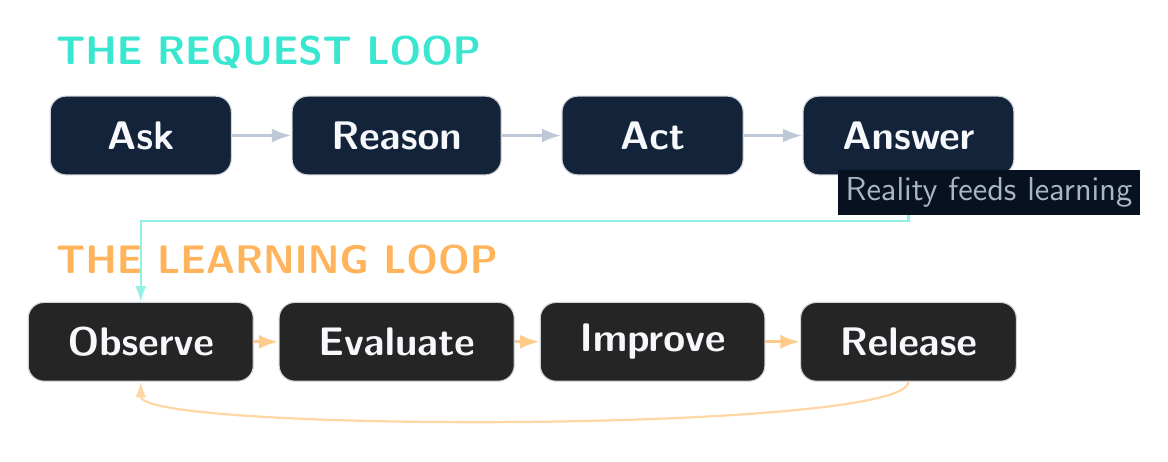
\begin{tikzpicture}[x=1cm,y=1cm]
    \node[anchor=west,text=Cyan,font=\fontsize{14}{17}\selectfont\bfseries] at (0,5.25) {THE REQUEST LOOP};
    \node[nodebase,minimum width=2.3cm] (ask) at (1.2,4.20) {Ask};
    \node[nodebase,minimum width=2.3cm] (reason) at (4.45,4.20) {Reason};
    \node[nodebase,minimum width=2.3cm] (act) at (7.70,4.20) {Act};
    \node[nodebase,minimum width=2.3cm] (answer) at (10.95,4.20) {Answer};
    \draw[flowarrow] (ask) -- (reason);
    \draw[flowarrow] (reason) -- (act);
    \draw[flowarrow] (act) -- (answer);

    \node[anchor=west,text=Orange,font=\fontsize{14}{17}\selectfont\bfseries] at (0,2.62) {THE LEARNING LOOP};
    \node[nodebase,minimum width=2.3cm,fill=Orange!12!Ink] (observe) at (1.2,1.58) {Observe};
    \node[nodebase,minimum width=2.3cm,fill=Orange!12!Ink] (evaluate) at (4.45,1.58) {Evaluate};
    \node[nodebase,minimum width=2.3cm,fill=Orange!12!Ink] (improve) at (7.70,1.58) {Improve};
    \node[nodebase,minimum width=2.3cm,fill=Orange!12!Ink] (release) at (10.95,1.58) {Release};
    \draw[flowarrow,draw=Orange!70] (observe) -- (evaluate);
    \draw[flowarrow,draw=Orange!70] (evaluate) -- (improve);
    \draw[flowarrow,draw=Orange!70] (improve) -- (release);
    \draw[thinflow,draw=Orange!55] (release.south) .. controls +(0,-0.65) and +(0,-0.65) .. (observe.south);

    \draw[thinflow,draw=Cyan!55] (answer.south) -- ++(0,-0.58) -| (observe.north);
    \node[anchor=east,text=Mist,fill=Ink,inner sep=1mm,font=\fontsize{13}{16}\selectfont] at (13.90,3.48) {Reality feeds learning};
  \end{tikzpicture}
\end{frame}

% -----------------------------------------------------------------------------
% 05 — Ambiguity
% -----------------------------------------------------------------------------
\sectionframe{01 / Intent}{Ambiguity is the\\first outage.}

\begin{frame}{Make intent executable}
  \vspace{0.10cm}
  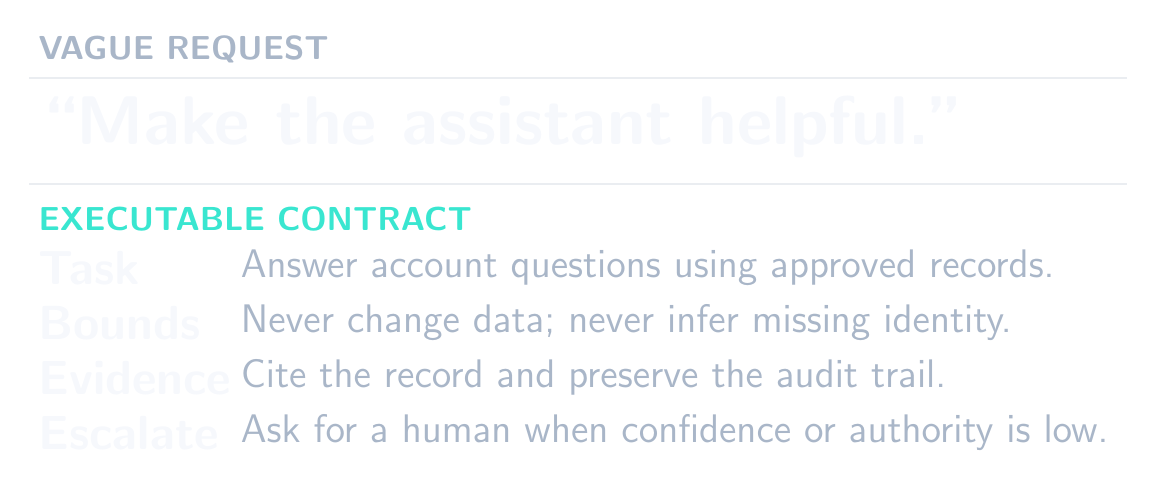
\begin{tikzpicture}[x=1cm,y=1cm]
    \draw[Mist!25,line width=0.8pt] (0.15,4.95) -- (14.1,4.95);
    \node[anchor=west,text=Mist,font=\fontsize{13}{16}\selectfont\bfseries] at (0.15,5.30) {VAGUE REQUEST};
    \node[anchor=west,text=Cloud,font=\fontsize{23}{28}\selectfont\bfseries] at (0.15,4.32) {``Make the assistant helpful.''};

    \draw[Mist!25,line width=0.8pt] (0.15,3.60) -- (14.1,3.60);
    \node[anchor=west,text=Cyan,font=\fontsize{13}{16}\selectfont\bfseries] at (0.15,3.16) {EXECUTABLE CONTRACT};

    \node[anchor=west,text=Cloud,font=\fontsize{16}{19}\selectfont\bfseries] at (0.15,2.54) {Task};
    \node[anchor=west,text=Mist,font=\fontsize{15}{18}\selectfont] at (2.72,2.54) {Answer account questions using approved records.};

    \node[anchor=west,text=Cloud,font=\fontsize{16}{19}\selectfont\bfseries] at (0.15,1.84) {Bounds};
    \node[anchor=west,text=Mist,font=\fontsize{15}{18}\selectfont] at (2.72,1.84) {Never change data; never infer missing identity.};

    \node[anchor=west,text=Cloud,font=\fontsize{16}{19}\selectfont\bfseries] at (0.15,1.14) {Evidence};
    \node[anchor=west,text=Mist,font=\fontsize{15}{18}\selectfont] at (2.72,1.14) {Cite the record and preserve the audit trail.};

    \node[anchor=west,text=Cloud,font=\fontsize{16}{19}\selectfont\bfseries] at (0.15,0.44) {Escalate};
    \node[anchor=west,text=Mist,font=\fontsize{15}{18}\selectfont] at (2.72,0.44) {Ask for a human when confidence or authority is low.};
  \end{tikzpicture}
\end{frame}

% -----------------------------------------------------------------------------
% 07 — Trust signals
% -----------------------------------------------------------------------------
\sectionframe{02 / Evidence}{Trust is a property\\of the whole system.}

\begin{frame}{Four signals reveal trust}
  \vspace{0.10cm}
  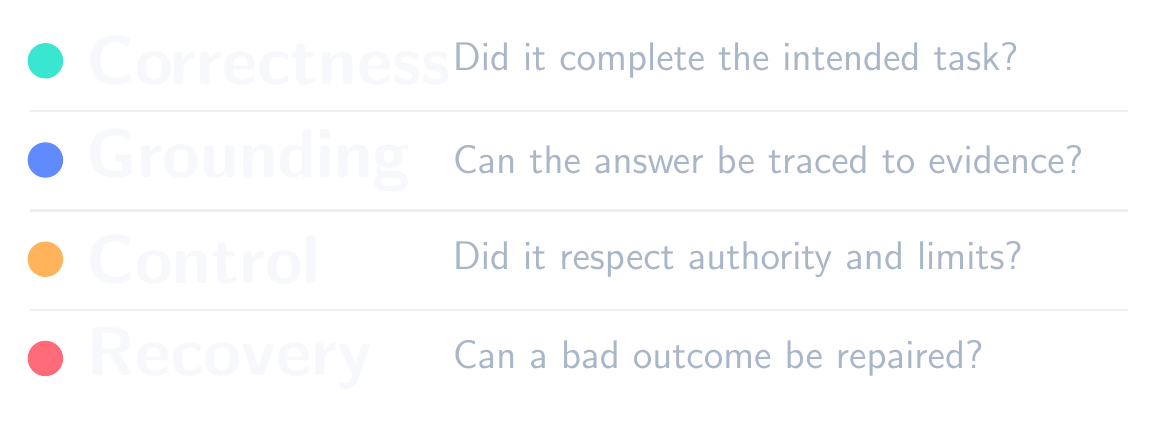
\begin{tikzpicture}[x=1cm,y=1cm]
    \node[dot,fill=Cyan] at (0.35,4.64) {};
    \node[anchor=west,text=Cloud,font=\fontsize{23}{27}\selectfont\bfseries] at (0.75,4.64) {Correctness};
    \node[anchor=west,text=Mist,font=\fontsize{15}{18}\selectfont] at (5.40,4.64) {Did it complete the intended task?};

    \node[dot,fill=Blue] at (0.35,3.38) {};
    \node[anchor=west,text=Cloud,font=\fontsize{23}{27}\selectfont\bfseries] at (0.75,3.38) {Grounding};
    \node[anchor=west,text=Mist,font=\fontsize{15}{18}\selectfont] at (5.40,3.38) {Can the answer be traced to evidence?};

    \node[dot,fill=Orange] at (0.35,2.12) {};
    \node[anchor=west,text=Cloud,font=\fontsize{23}{27}\selectfont\bfseries] at (0.75,2.12) {Control};
    \node[anchor=west,text=Mist,font=\fontsize{15}{18}\selectfont] at (5.40,2.12) {Did it respect authority and limits?};

    \node[dot,fill=Coral] at (0.35,0.86) {};
    \node[anchor=west,text=Cloud,font=\fontsize{23}{27}\selectfont\bfseries] at (0.75,0.86) {Recovery};
    \node[anchor=west,text=Mist,font=\fontsize{15}{18}\selectfont] at (5.40,0.86) {Can a bad outcome be repaired?};

    \draw[Mist!22,line width=0.8pt] (0.15,4.00) -- (14.1,4.00);
    \draw[Mist!22,line width=0.8pt] (0.15,2.74) -- (14.1,2.74);
    \draw[Mist!22,line width=0.8pt] (0.15,1.48) -- (14.1,1.48);
  \end{tikzpicture}
\end{frame}

% -----------------------------------------------------------------------------
% 09 — Evaluation
% -----------------------------------------------------------------------------
\begin{frame}{Evaluate real behavior}
  \vspace{0.12cm}
  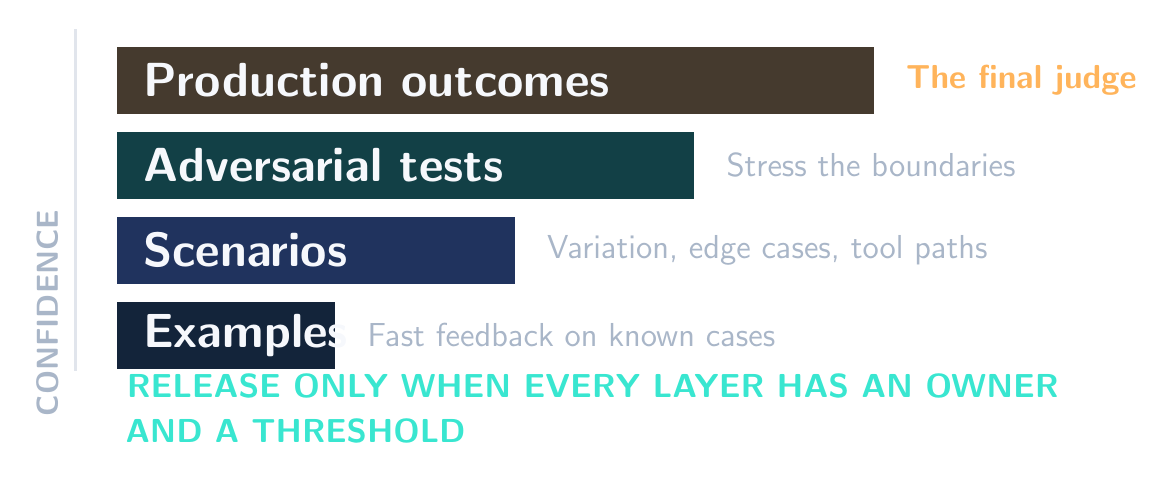
\begin{tikzpicture}[x=0.95cm,y=1cm]
    \draw[Mist!35,line width=1pt] (0.55,0.68) -- (0.55,5.02);
    \node[anchor=east,rotate=90,text=Mist,font=\fontsize{11}{13}\selectfont\bfseries] at (0.17,2.85) {CONFIDENCE};

    \fill[Panel] (1.10,0.70) rectangle (4.02,1.55);
    \node[anchor=west,text=Cloud,font=\fontsize{17}{20}\selectfont\bfseries] at (1.32,1.13) {Examples};
    \node[anchor=west,text=Mist,font=\fontsize{13}{16}\selectfont] at (4.32,1.13) {Fast feedback on known cases};

    \fill[Blue!28!Ink] (1.10,1.78) rectangle (6.42,2.63);
    \node[anchor=west,text=Cloud,font=\fontsize{17}{20}\selectfont\bfseries] at (1.32,2.21) {Scenarios};
    \node[anchor=west,text=Mist,font=\fontsize{13}{16}\selectfont] at (6.72,2.21) {Variation, edge cases, tool paths};

    \fill[Cyan!22!Ink] (1.10,2.86) rectangle (8.82,3.71);
    \node[anchor=west,text=Cloud,font=\fontsize{17}{20}\selectfont\bfseries] at (1.32,3.29) {Adversarial tests};
    \node[anchor=west,text=Mist,font=\fontsize{13}{16}\selectfont] at (9.12,3.29) {Stress the boundaries};

    \fill[Orange!25!Ink] (1.10,3.94) rectangle (11.22,4.79);
    \node[anchor=west,text=Cloud,font=\fontsize{17}{20}\selectfont\bfseries] at (1.32,4.37) {Production outcomes};
    \node[anchor=west,text=Orange,font=\fontsize{13}{16}\selectfont\bfseries] at (11.52,4.37) {The final judge};

    \node[anchor=west,text=Cyan,text width=12.0cm,font=\fontsize{13}{16}\selectfont\bfseries] at (1.10,0.20) {RELEASE ONLY WHEN EVERY LAYER HAS AN OWNER AND A THRESHOLD};
  \end{tikzpicture}
\end{frame}

% -----------------------------------------------------------------------------
% 10 — Observability
% -----------------------------------------------------------------------------
\begin{frame}{Production must explain}
  \vspace{0.10cm}
  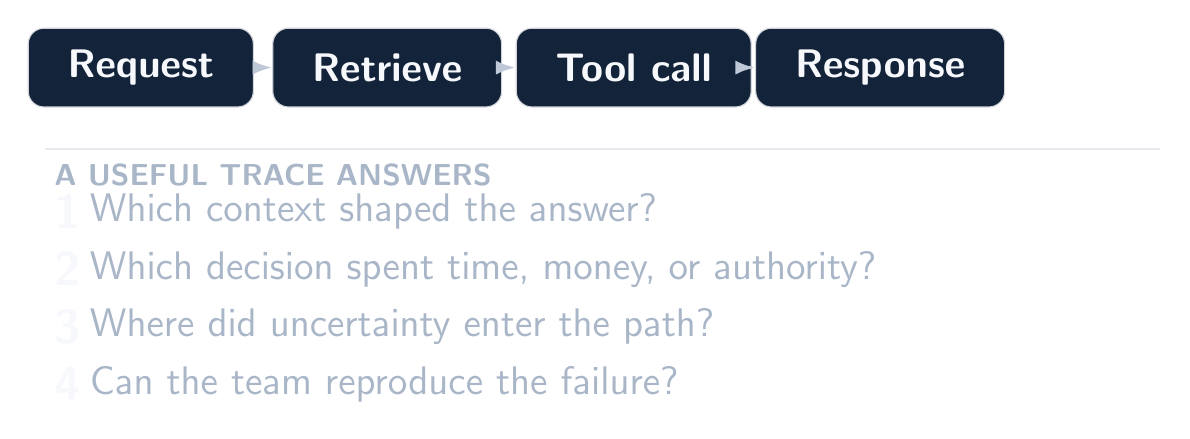
\begin{tikzpicture}[x=1cm,y=1cm]
    \node[nodebase,minimum width=2.45cm] (prompt) at (1.25,4.38) {Request};
    \node[nodebase,minimum width=2.45cm] (retrieve) at (4.38,4.38) {Retrieve};
    \node[nodebase,minimum width=2.45cm] (tool) at (7.51,4.38) {Tool call};
    \node[nodebase,minimum width=2.45cm] (response) at (10.64,4.38) {Response};
    \draw[flowarrow] (prompt) -- (retrieve);
    \draw[flowarrow] (retrieve) -- (tool);
    \draw[flowarrow] (tool) -- (response);

    \draw[Mist!28,line width=0.8pt] (0.03,3.35) -- (14.2,3.35);
    \node[anchor=west,text=Mist,font=\fontsize{11}{13}\selectfont\bfseries] at (0.03,3.02) {A USEFUL TRACE ANSWERS};

    \node[anchor=west,text=Cloud,font=\fontsize{16}{19}\selectfont\bfseries] at (0.03,2.55) {1};
    \node[anchor=west,text=Mist,font=\fontsize{15}{18}\selectfont] at (0.48,2.55) {Which context shaped the answer?};

    \node[anchor=west,text=Cloud,font=\fontsize{16}{19}\selectfont\bfseries] at (0.03,1.82) {2};
    \node[anchor=west,text=Mist,font=\fontsize{15}{18}\selectfont] at (0.48,1.82) {Which decision spent time, money, or authority?};

    \node[anchor=west,text=Cloud,font=\fontsize{16}{19}\selectfont\bfseries] at (0.03,1.09) {3};
    \node[anchor=west,text=Mist,font=\fontsize{15}{18}\selectfont] at (0.48,1.09) {Where did uncertainty enter the path?};

    \node[anchor=west,text=Cloud,font=\fontsize{16}{19}\selectfont\bfseries] at (0.03,0.36) {4};
    \node[anchor=west,text=Mist,font=\fontsize{15}{18}\selectfont] at (0.48,0.36) {Can the team reproduce the failure?};
  \end{tikzpicture}
\end{frame}

% -----------------------------------------------------------------------------
% 11 — Failure budgets
% -----------------------------------------------------------------------------
\begin{frame}{Give failure a budget}
  \vspace{0.08cm}
  \begin{columns}[T,onlytextwidth]
    \begin{column}{0.48\textwidth}
      \eyebrow{One operating equation}\par\vspace{0.32cm}
      {\color{Cloud}\fontsize{17}{22}\selectfont
      \[
        \text{risk burn} =
        \frac{\text{weighted failures}}{\text{allowed failures}}
      \]
      }
      \mutedtext{Weight errors by consequence, not by how easy they are to count.}
    \end{column}
    \hfill
    \begin{column}{0.47\textwidth}
      \eyebrow{When the budget burns}\par\vspace{0.42cm}
      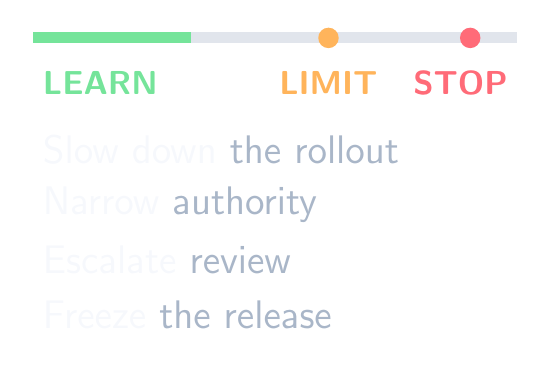
\begin{tikzpicture}[x=1cm,y=1cm]
        \draw[Mist!35,line width=4pt] (0,3.55) -- (6.15,3.55);
        \draw[Green,line width=4pt] (0,3.55) -- (2.0,3.55);
        \fill[Orange] (3.75,3.55) circle (0.13);
        \fill[Coral] (5.55,3.55) circle (0.13);
        \node[anchor=west,text=Green,font=\fontsize{13}{16}\selectfont\bfseries] at (0,2.98) {LEARN};
        \node[anchor=center,text=Orange,font=\fontsize{13}{16}\selectfont\bfseries] at (3.75,2.98) {LIMIT};
        \node[anchor=east,text=Coral,font=\fontsize{13}{16}\selectfont\bfseries] at (6.15,2.98) {STOP};

        \node[anchor=west,text=Mist,font=\fontsize{14}{17}\selectfont] at (0,2.13) {\textcolor{Cloud}{Slow down} the rollout};
        \node[anchor=west,text=Mist,font=\fontsize{14}{17}\selectfont] at (0,1.43) {\textcolor{Cloud}{Narrow} authority};
        \node[anchor=west,text=Mist,font=\fontsize{14}{17}\selectfont] at (0,0.73) {\textcolor{Cloud}{Escalate} review};
        \node[anchor=west,text=Mist,font=\fontsize{14}{17}\selectfont] at (0,0.03) {\textcolor{Cloud}{Freeze} the release};
      \end{tikzpicture}
    \end{column}
  \end{columns}
\end{frame}

% -----------------------------------------------------------------------------
% 12 — Human control
% -----------------------------------------------------------------------------
\sectionframe{03 / Control}{A human should have\\authority, not homework.}

\begin{frame}{Human intervention}
  \vspace{0.10cm}
  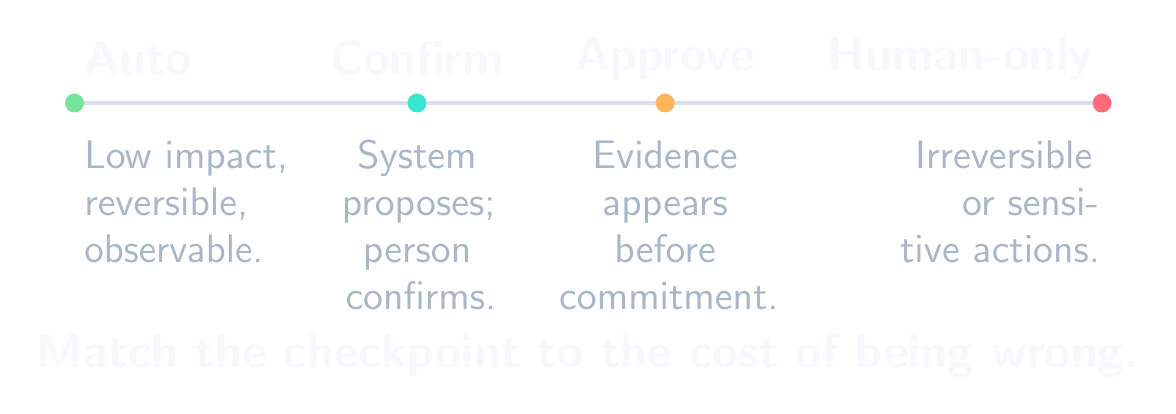
\begin{tikzpicture}[x=1cm,y=1cm]
    \draw[Mist!42,line width=1.3pt] (0.60,3.78) -- (13.65,3.78);
    \foreach \x/\c in {0.60/Green,4.95/Cyan,8.10/Orange,13.65/Coral}{\fill[\c] (\x,3.78) circle (0.12);}

    \node[anchor=west,text=Cloud,font=\fontsize{19}{23}\selectfont\bfseries] at (0.60,4.35) {Auto};
    \node[anchor=center,text=Cloud,font=\fontsize{19}{23}\selectfont\bfseries] at (4.95,4.35) {Confirm};
    \node[anchor=center,text=Cloud,font=\fontsize{19}{23}\selectfont\bfseries] at (8.10,4.35) {Approve};
    \node[anchor=east,text=Cloud,font=\fontsize{19}{23}\selectfont\bfseries] at (13.65,4.35) {Human-only};

    \node[anchor=north west,text=Mist,text width=2.75cm,font=\fontsize{14}{17}\selectfont] at (0.60,3.42) {Low impact, reversible, observable.};
    \node[anchor=north,text=Mist,text width=2.75cm,align=center,font=\fontsize{14}{17}\selectfont] at (4.95,3.42) {System proposes; person confirms.};
    \node[anchor=north,text=Mist,text width=2.75cm,align=center,font=\fontsize{14}{17}\selectfont] at (8.10,3.42) {Evidence appears before commitment.};
    \node[anchor=north east,text=Mist,text width=2.75cm,align=right,font=\fontsize{14}{17}\selectfont] at (13.65,3.42) {Irreversible or sensitive actions.};

    \node[anchor=south,text=Cloud,font=\fontsize{17}{21}\selectfont\bfseries] at (7.12,0.18) {Match the checkpoint to the cost of being wrong.};
  \end{tikzpicture}
\end{frame}

% -----------------------------------------------------------------------------
% 14 — Architecture
% -----------------------------------------------------------------------------
\begin{frame}{Reduce the blast radius}
  \vspace{0.08cm}
  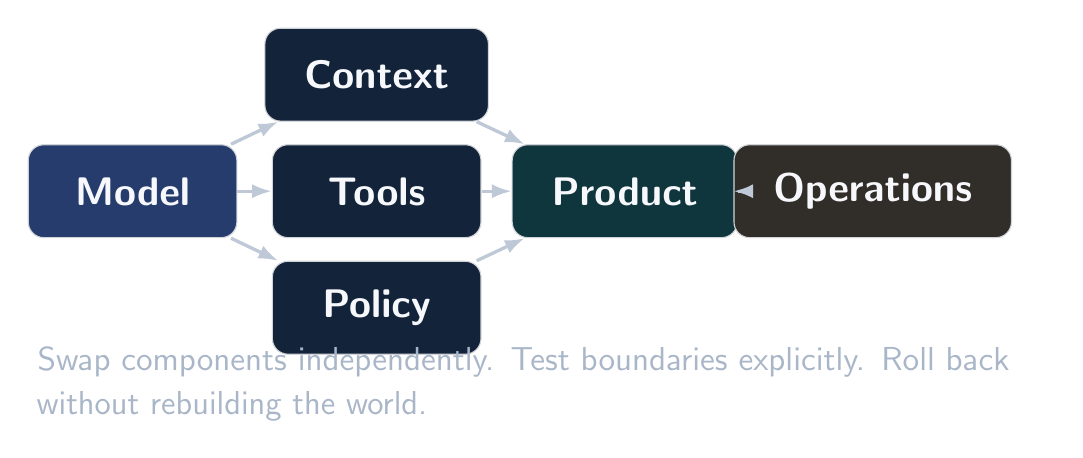
\begin{tikzpicture}[x=1cm,y=1cm]
    \node[nodebase,minimum width=2.65cm,minimum height=1.18cm,fill=Blue!35!Ink] (model) at (2.0,2.77) {Model};
    \node[nodebase,minimum width=2.65cm,minimum height=1.18cm] (context) at (5.10,4.25) {Context};
    \node[nodebase,minimum width=2.65cm,minimum height=1.18cm] (tools) at (5.10,2.77) {Tools};
    \node[nodebase,minimum width=2.65cm,minimum height=1.18cm] (policy) at (5.10,1.29) {Policy};
    \node[nodebase,minimum width=2.65cm,minimum height=1.18cm,fill=Cyan!17!Ink] (product) at (8.25,2.77) {Product};
    \node[nodebase,minimum width=2.65cm,minimum height=1.18cm,fill=Orange!17!Ink] (ops) at (11.40,2.77) {Operations};

    \draw[flowarrow] (model) -- (context);
    \draw[flowarrow] (model) -- (tools);
    \draw[flowarrow] (model) -- (policy);
    \draw[flowarrow] (context) -- (product);
    \draw[flowarrow] (tools) -- (product);
    \draw[flowarrow] (policy) -- (product);
    \draw[flowarrow] (product) -- (ops);

    \node[anchor=west,text=Mist,text width=12.8cm,font=\fontsize{13}{16}\selectfont] at (0.67,0.32)
      {Swap components independently. Test boundaries explicitly. Roll back without rebuilding the world.};
  \end{tikzpicture}
\end{frame}

% -----------------------------------------------------------------------------
% 15 — Thin slice
% -----------------------------------------------------------------------------
\begin{frame}{Ship one thin vertical slice}
  \vspace{0.10cm}
  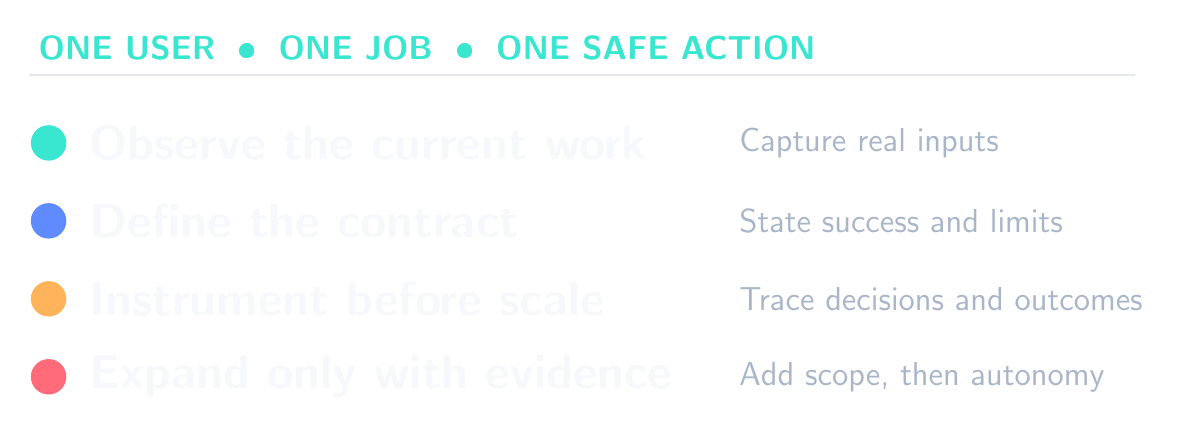
\begin{tikzpicture}[x=1cm,y=1cm]
    \node[anchor=west,text=Cyan,font=\fontsize{13}{16}\selectfont\bfseries] at (0.10,4.82) {ONE USER \;\textbullet\; ONE JOB \;\textbullet\; ONE SAFE ACTION};
    \draw[Mist!30,line width=0.9pt] (0.10,4.48) -- (14.15,4.48);

    \node[dot,fill=Cyan] at (0.35,3.62) {};
    \node[anchor=west,text=Cloud,font=\fontsize{18}{22}\selectfont\bfseries] at (0.75,3.62) {Observe the current work};
    \node[anchor=west,text=Mist,font=\fontsize{12}{15}\selectfont] at (9.00,3.62) {Capture real inputs};

    \node[dot,fill=Blue] at (0.35,2.63) {};
    \node[anchor=west,text=Cloud,font=\fontsize{18}{22}\selectfont\bfseries] at (0.75,2.63) {Define the contract};
    \node[anchor=west,text=Mist,font=\fontsize{12}{15}\selectfont] at (9.00,2.63) {State success and limits};

    \node[dot,fill=Orange] at (0.35,1.64) {};
    \node[anchor=west,text=Cloud,font=\fontsize{18}{22}\selectfont\bfseries] at (0.75,1.64) {Instrument before scale};
    \node[anchor=west,text=Mist,font=\fontsize{12}{15}\selectfont] at (9.00,1.64) {Trace decisions and outcomes};

    \node[dot,fill=Coral] at (0.35,0.65) {};
    \node[anchor=west,text=Cloud,font=\fontsize{18}{22}\selectfont\bfseries] at (0.75,0.65) {Expand only with evidence};
    \node[anchor=west,text=Mist,font=\fontsize{12}{15}\selectfont] at (9.00,0.65) {Add scope, then autonomy};
  \end{tikzpicture}
\end{frame}

% -----------------------------------------------------------------------------
% 16 — Operating loop in code
% -----------------------------------------------------------------------------
\begin{frame}[fragile]{The operating loop}
  \begin{beamercolorbox}[wd=\textwidth,sep=0.18cm,leftskip=0.18cm,rightskip=0.18cm]{code panel}
    
\begin{tikzpicture}
      \fill[Coral] (0,0) circle (0.07);
      \fill[Orange] (0.26,0) circle (0.07);
      \fill[Green] (0.52,0) circle (0.07);
      \node[anchor=west,text=Mist,font=\fontsize{11}{13}\selectfont\bfseries] at (0.83,0) {release-loop.py};
    \end{tikzpicture}
    \vspace{0.20cm}
    \begin{lstlisting}[style=keynote]
contract = define(task, bounds, evidence, escalation)
candidate = system.run(request, contract)
trace = observe(candidate)
score = evaluate(trace, contract)
if score.within_budget():
    release(candidate)
else:
    narrow_authority()
    learn(trace)
    \end{lstlisting}
  \end{beamercolorbox}
\end{frame}

% -----------------------------------------------------------------------------
% 17 — Runway
% -----------------------------------------------------------------------------
\begin{frame}{Six weeks to evidence}
  \vspace{0.10cm}
  \resizebox{0.99\textwidth}{!}{%
  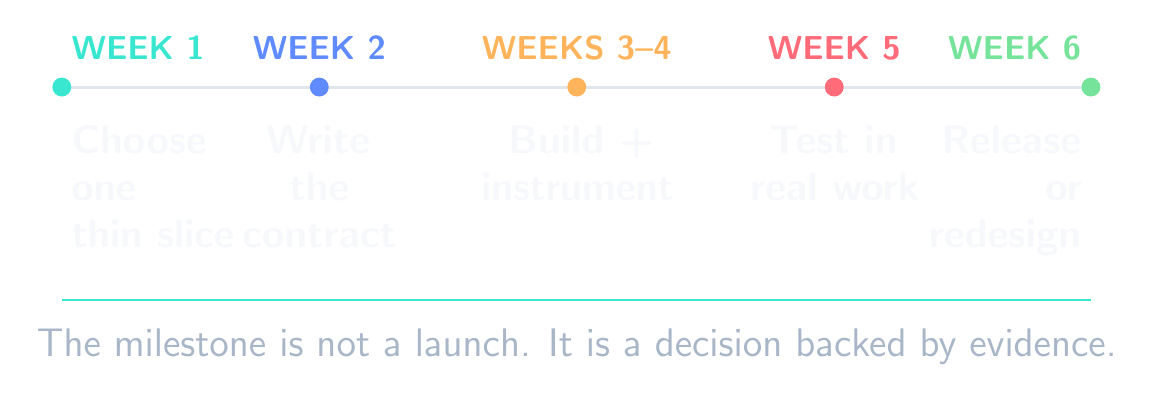
\begin{tikzpicture}[x=1cm,y=1cm]
    \draw[Mist!35,line width=1.1pt] (0.55,3.83) -- (13.62,3.83);
    \foreach \x/\c in {0.55/Cyan,3.82/Blue,7.09/Orange,10.36/Coral,13.62/Green}{\fill[\c] (\x,3.83) circle (0.12);}

    \node[anchor=south west,text=Cyan,font=\fontsize{12}{14}\selectfont\bfseries] at (0.55,4.05) {WEEK 1};
    \node[anchor=south,text=Blue,font=\fontsize{12}{14}\selectfont\bfseries] at (3.82,4.05) {WEEK 2};
    \node[anchor=south,text=Orange,font=\fontsize{12}{14}\selectfont\bfseries] at (7.09,4.05) {WEEKS 3--4};
    \node[anchor=south,text=Coral,font=\fontsize{12}{14}\selectfont\bfseries] at (10.36,4.05) {WEEK 5};
    \node[anchor=south east,text=Green,font=\fontsize{12}{14}\selectfont\bfseries] at (13.62,4.05) {WEEK 6};

    \node[anchor=north west,text=Cloud,text width=2.18cm,font=\fontsize{14}{17}\selectfont\bfseries] at (0.55,3.46) {Choose one\\thin slice};
    \node[anchor=north,text=Cloud,text width=2.18cm,align=center,font=\fontsize{14}{17}\selectfont\bfseries] at (3.82,3.46) {Write the\\contract};
    \node[anchor=north,text=Cloud,text width=2.42cm,align=center,font=\fontsize{14}{17}\selectfont\bfseries] at (7.09,3.46) {Build +\\instrument};
    \node[anchor=north,text=Cloud,text width=2.18cm,align=center,font=\fontsize{14}{17}\selectfont\bfseries] at (10.36,3.46) {Test in\\real work};
    \node[anchor=north east,text=Cloud,text width=2.18cm,align=right,font=\fontsize{14}{17}\selectfont\bfseries] at (13.62,3.46) {Release or\\redesign};

    \draw[Cyan,line width=0.8pt] (0.55,1.13) -- (13.62,1.13);
    \node[anchor=north,text=Mist,font=\fontsize{15}{18}\selectfont] at (7.09,0.88)
      {The milestone is not a launch. It is a decision backed by evidence.};
  \end{tikzpicture}%
  }
\end{frame}

% -----------------------------------------------------------------------------
% 18 — Questions leaders should ask
% -----------------------------------------------------------------------------
\begin{frame}{Questions before scale}
  \vspace{0.10cm}
  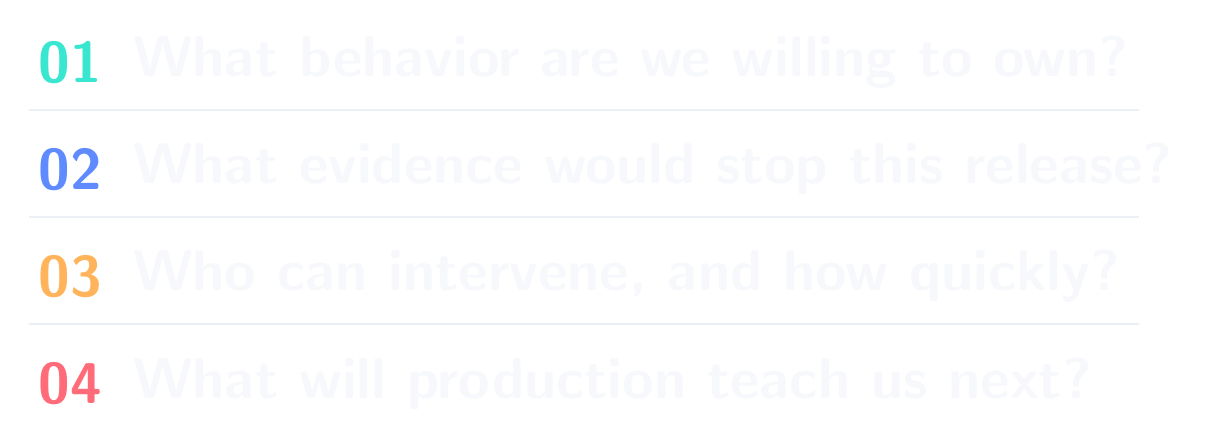
\begin{tikzpicture}[x=1cm,y=1cm]
    \node[anchor=west,text=Cyan,font=\fontsize{22}{27}\selectfont\bfseries] at (0.05,4.70) {01};
    \node[anchor=west,text=Cloud,font=\fontsize{20}{24}\selectfont\bfseries] at (1.25,4.70) {What behavior are we willing to own?};
    \draw[Mist!22,line width=0.8pt] (0.05,4.10) -- (14.15,4.10);

    \node[anchor=west,text=Blue,font=\fontsize{22}{27}\selectfont\bfseries] at (0.05,3.34) {02};
    \node[anchor=west,text=Cloud,font=\fontsize{20}{24}\selectfont\bfseries] at (1.25,3.34) {What evidence would stop this release?};
    \draw[Mist!22,line width=0.8pt] (0.05,2.74) -- (14.15,2.74);

    \node[anchor=west,text=Orange,font=\fontsize{22}{27}\selectfont\bfseries] at (0.05,1.98) {03};
    \node[anchor=west,text=Cloud,font=\fontsize{20}{24}\selectfont\bfseries] at (1.25,1.98) {Who can intervene, and how quickly?};
    \draw[Mist!22,line width=0.8pt] (0.05,1.38) -- (14.15,1.38);

    \node[anchor=west,text=Coral,font=\fontsize{22}{27}\selectfont\bfseries] at (0.05,0.62) {04};
    \node[anchor=west,text=Cloud,font=\fontsize{20}{24}\selectfont\bfseries] at (1.25,0.62) {What will production teach us next?};
  \end{tikzpicture}
\end{frame}

% -----------------------------------------------------------------------------
% 19 — Close
% -----------------------------------------------------------------------------
\begin{frame}[plain,t]
  \begin{tikzpicture}[remember picture,overlay]
    \fill[Ink] (current page.south west) rectangle (current page.north east);
    \draw[Blue!34,line width=0.8pt]
      ([xshift=-0.75cm,yshift=0.75cm]current page.south east) circle (3.55cm);
    \draw[Cyan!32,line width=0.8pt]
      ([xshift=-0.75cm,yshift=0.75cm]current page.south east) circle (2.62cm);
    \draw[Orange!30,line width=0.8pt]
      ([xshift=-0.75cm,yshift=0.75cm]current page.south east) circle (1.68cm);
  \end{tikzpicture}
  \vspace*{0.74cm}
  \eyebrow{The standard for what comes next}\par\vspace{0.55cm}
  {\color{Cloud}\bfseries\fontsize{47}{52}\selectfont
    Ship \cyantext{evidence},\\not confidence.\par}
  \vspace{0.54cm}
  {\color{Mist}\fontsize{19}{24}\selectfont
    Define the contract. Instrument the path.\\
    Earn autonomy one verified outcome at a time.\par}
  \begin{tikzpicture}[remember picture,overlay]
    \node[anchor=south west,text=Cyan,font=\bfseries\fontsize{13}{16}\selectfont]
      at ([xshift=0.78cm,yshift=0.16cm]current page.south west) {BEYOND THE DEMO};
  \end{tikzpicture}
\end{frame}

\end{document}
